\begin{flushleft}
    \huge
    \textbf{2. Analysis}
    \vspace{0.1cm}

    \Large
    \begin{enumerate}
        \item {\Large Statement of Investigation} \\
            \large
            \vspace{0.2cm}
            I plan to investigate Machine Learning by developing a survival simulation environment 
            in which a character will be controlled by a Machine Learning algorithm. The survival simulation will 
            present multiple challenges such as dynamic threats towards the agent in order to provide a complex 
            problem for it to solve. The key question I aim to answer with this investigation is:

            \vspace{0.3cm}

            \begin{center}
            \textbf{Can you train a Machine Learning algorithm to survive in a pseudo random, open-world environment?}
            \end{center}

            \vspace{0.3cm}

            I find this question to be quite interesting because there is multiple layers of complexity to it, 
            with several different problems to solve. Answering the question will require me to dive headfirst into 
            Machine Learning picking things up as fast as possible.

        \vspace{1cm}
        \item {\Large Background} \\
            \vspace{0.2cm}
            I am investigating this area of Computer Science because I've been interesting in attempting a form of
            Machine Learning for a while now but havent had a reason to dive into it. Machine Learning is an evolving
            field, with mere infinite applications such as Image Recognition, Chat Bots, Self Driving Cars, 
            etc. I feel as though my project will be sufficiently advanced enough to expand my knowledge of the subject.
            It will require lots of research, planning, and design work in order to successfully fulfil my Technical
            Solution. \\
            \vspace{0.2cm}

        \vspace{1cm}
        \item {\Large Expert} \\
            \vspace{0.2cm}
            For my expert I approached one of my friends, Ben, who has prior experience with Machine Learning. He has
            created his own Hand Written Digit Recognition Network before, along with using Python Libraries such as 
            \textit{PyTorch} to train an agent to play the game \textit{Flappy Bird}, among other ML projects. He has 
            a much better understanding of Machine Learning than me currently, so hopefully he will be a good resource 
            as I develop my project. \\
            \vspace{0.2cm}
            He has agreed to answer some questions for my Interview once I have completed my Initial Investigation.

        \vspace{1cm}
        \item {\Large Initial Research} \\
            \begin{enumerate}
                \item {\Large Existing Investigations} \\
                    \large
                    \vspace{0.2cm}

                \item {\Large Algorithms and Potential Data Types} \\
                    \large
                    \vspace{0.2cm}
                    As part of developing a Machine Learning Algorithm, I will need to implement a Matrix class in order to
                    implement a neural network. Matrices are commonly used to represent individual layers of a network. Along
                    with making calculations much easier, condensing them into performing operations on matrices, rather than
                    nested using nested for loops and lists. As part of my Initial Research I have taken the time to understand
                    how a Neural Network functions, it turns out I have already learned most of the maths needed to understand
                    how it works in my A Level Maths and Further Maths courses. \\
                    \vspace{0.2cm}
                    A Neural Network functions as a series mathematical equations used to recognise relationships between inputs
                    and desired outputs. They take in a Vector of Input Data, and output a Vector of Output Data. They can be
                    in simple terms as a function: $N(x)$ where: $\{x \in V, N(x) \in V\}$. The functions name in this case is
                    Forward Propagation. 
                    \vspace{0.2cm}
                    We form a Neural Network with multiple layers of Nodes, the layers being referred to as the Input Layer, 
                    Hidden Layer/s and Output Layer. In this case each Node is connected to every Node in the previous layer and
                    the following layer. In the below image is represented a Neural Network with a layer structure of $[3, 5, 2]$.

                    \vspace{0.1cm}
                    \centerline{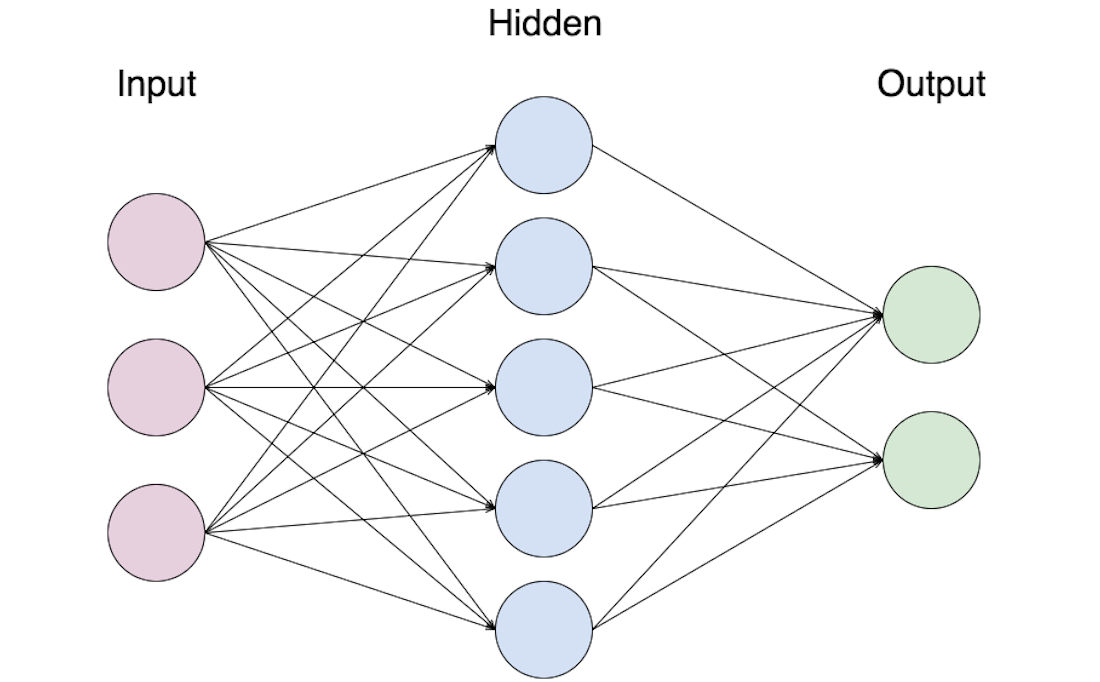
\includegraphics[width=10cm]{Images/Initial Research/NeuralNetworkExample.png}}

                    Each connection, otherwise known as an Arc or Edge, has an associated weight. Along with every output of a
                    layer having an associated Bias. These are used to compute the outcome of a network.
                    \vspace{0.2cm}
                    Forward Propagation is used to compute the outcome of a network, it has a general form and uses Matrix
                    Multiplication and Addition to achieve this.

                
                \item {\Large Interview} \\
                    \large
                    \vspace{0.2cm}
            \end{enumerate}

            \pagebreak
        \item {\Large Prototype} \\
            \large
            \vspace{0.2cm}
            Before starting my Prototype I had to decide upon a short list of objectives I wanted to 
            complete/investigate as part of it. These boiled down to a few things:

            \vspace{0.2cm}
            \begin{enumerate}
                \item Terrain Generation
                \item Displaying the Generated Terrain using a Grahics Library
                \item Matrix and Vector implementation
            \end{enumerate}
            \vspace{0.2cm}

            For my Prototype, I first created a GitHub Repository, available here: 
            
            \vspace{0.1cm}
            \centerline{\textit{https://github.com/TheTacBanana/CompSciNEAPrototype}}
            \vspace{0.1cm}

            I had created a hierarchy of importance for development in my head, visualized using this flow diagram:

            \begin{center}
                \begin{tikzpicture}
                    \matrix (m)[matrix of nodes, column  sep=0.5cm,row  sep=0.5cm, align=center, nodes={rectangle,draw, anchor=center} ]{
                        |[block]| Creating a window with Graphics Library &  |[block]| Display Generated Terrain \\   
                        |[block]| Generate Terrain using a pseudorandom algorithm &  |[block]| Store Terrain to 2d List \\
                        |[block]| Create a Matrix Data Structure & |[block]| Create a Vector Data Structure which inherits from Matrix \\
                        |[block]| Create Operation Methods for the Data Structure & \\
                    };
                    \path [>=latex,->] (m-1-1) edge (m-1-2);
                    \path [>=latex,<-] (m-1-2) edge (m-2-2);
                    \path [>=latex,->] (m-2-1) edge (m-2-2);
                    \path [>=latex,->] (m-3-1) edge (m-3-2);
                    \path [>=latex,->] (m-3-1) edge (m-4-1);
                \end{tikzpicture}
            \end{center}

            I decided to use Python for developing my Prototype, this seemed like a good fit due to me 
            having lots of experience with the language. Python is a Dynamically Typed and Interpretted 
            language which makes it versatile for protyping and fast, iterative development.
            
            \vspace{0.5cm}

            {\Large Terrain Generation and Displaying} \\
            \vspace{0.25cm}

            Starting from the begining of my hierarchy I installed Pygame using \textit{pip} and started creating a window.
            This was a relatively simple task only taking a few lines:
            \vspace{0.5cm}

            \normalsize
            \begin{lstlisting}[language=Python]
import pygame

simSize = 128
gridSize = 2

window = pygame.display.set_mode((simSize*gridSize, simSize*gridSize))
pygame.display.set_caption("Procedural Generation")

running = True
while running == True:
  for event in pygame.event.get():
    if event.type == pygame.QUIT:
      running = False
            \end{lstlisting}

            \vspace{0.5cm}

            \large
            This creates a window like this: \\ 
            \vspace{0.5cm}
            \centerline{
\includegraphics{Images/Prototype/CreateWindowExample.PNG}}

            \vspace{0.5cm}

            Following the hierarchy I then added noise generation by generating random numbers and 
            assigning them to a 2d List. Shown here: 
            
            \normalsize\begin{lstlisting}[language=Python]
def GenerateMap(self, seed):
    random.seed(seed)
    for y in range(0, self.arraySize):
        for x in range(0, self.arraySize):
            self.heightArray[x][y] = round(random.random(),2)
            \end{lstlisting}

            \vspace{0.5cm}

            \large
            After creating some code to draw squares based upon the random value, I ended up with this 
            random array of Black-White squares:\\
            \vspace{0.5cm}
            \centerline{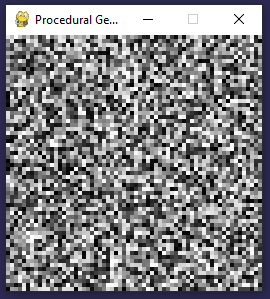
\includegraphics{Images/Prototype/RandomNoiseExample.PNG}}

            \vspace{0.5cm}

            This was a good start, but didnt really look like terrain yet. As part of my research I came 
            across simple algorithms to turn random noise into usable 2d terrain. I decided to implement
            these algorithms. They are relatively short and didnt take too much time to implement. I've
            named the two algorithms UpDownNeutralGen and Average.

            \vspace{1cm}

            {\large UpDownNeutralGen Method} \\
            \vspace{0.25cm}

            The UpDownNeutralGen method takes a tile, and considers every tile around it. It sums the tile 
            which are greater than, less than, or within a certain range of the tile height. And then pulls
            the selected tile in the direction which has the highest precedence. As an example, here are some
            randomly generated values:

            \begin{center}
                \begin{tabular}{| C{0.75cm} | C{0.75cm} | C{0.75cm} |}
                    \hline
                    0.71 & 0.19 & 0.3 \\ [0.75cm]
                    \hline
                    0.46 & 0.26 & 0.82 \\ [0.75cm]
                    \hline
                    0.63 & 0.35 & 0.05 \\ [0.75cm]
                    \hline
                \end{tabular}
            \end{center}

            If we count the surrounding values into corresponding Higher, Lower and Neutral we get: \\

            \begin{center}
                \begin{tabular}{| M{2cm} | M{2cm} | M{2cm} |}
                    \hline
                    Higher & Lower & Neutral \\ [0.25cm]
                    \hline
                    4 & 1 & 3 \\ [0.25cm]
                    \hline
                \end{tabular}
            \end{center}

            \vspace{0.5cm}

            This leads us to calculating the \textit{pullValue}, respectively for each case:
            \begin{center}
                $Up -> pullValue = upTiles * 0.09$ \\
                $Down -> pullValue = upTiles * -0.08$ \\
                $Neutral -> pullValue = 0$ \\
                \vspace{0.5cm}
                $Value[x][y] \pluseq pullValue$\\
            \end{center}
            
            \vspace{0.5cm}

            We then add the pullValue to the original square value, leaving us with the updated value. The code for 
            this shown under the Prototype Code Header.
            \vspace{0.5cm}

            {\large Average Method}
            \vspace{0.25cm}

            The Average method takes a tile and considers every tile around it, this time instead of looking at the
            differences, it creates an average from the 8 surrounding tiles. It then sets the selected tile to this
            average value. As an example, here are some randomly generated values:

            \begin{center}
                \begin{tabular}{| C{0.75cm} | C{0.75cm} | C{0.75cm} |}
                    \hline
                    0.83 & 0.93 & 0.64 \\ [0.75cm]
                    \hline
                    0.07 & 0.38 & 0.21 \\ [0.75cm]
                    \hline
                    0.33 & 0.94 & 0.95 \\ [0.75cm]
                    \hline
                \end{tabular}
                \vspace{0.25cm}

                Summing these and dividing by the total grants us the average:

                \[
                \frac{0.83 + 0.93 + 0.64 + 0.07 + 0.38 + 0.21 + 0.95 + 0.33 + 0.94}{9} = 0.586
                \]
                $Value[x][y] = 0.586$
            \end{center}
            \vspace{0.25cm}

            The code for this shown under the Prototype Code Header.

            \vspace{1cm}

            {\large Finished Terrain Generation} \\
            \vspace{0.25cm}

            Overall I am happy with the Terrain generation, though I feel as if it could be improved to look more realistic.
            The difference between the original random noise and the Colour Mapped Terrain looks so much better.

            \begin{center}
                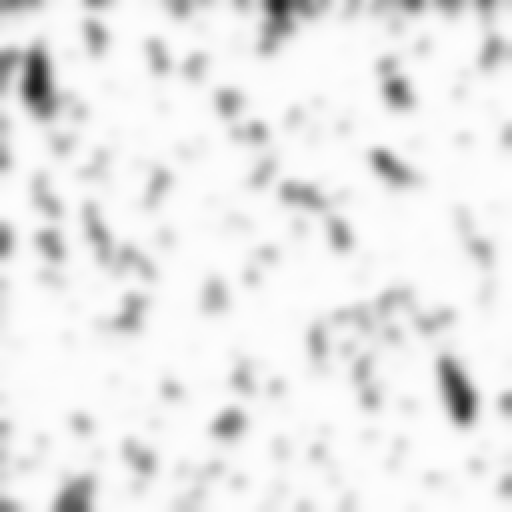
\includegraphics[width=6cm]{Images/Prototype/Seed420 Grayscale.png}
                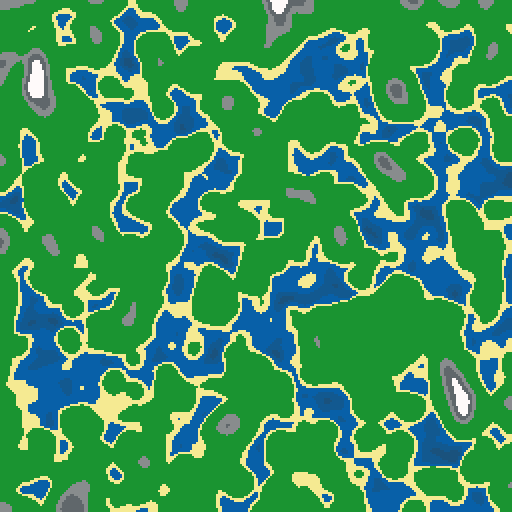
\includegraphics[width=6cm]{Images/Prototype/Seed420 Colour.png} 
            \end{center}
            
            \vspace{1cm}
            {\Large Matrix Data Structure} \\
            \vspace{0.25cm}

            As part of my Matrix Class I made a list of operations which would be key to a Matrix Class, along with being useful
            for Machine Learning. A Matrix is an abstract data type, commonly used in Maths, but has practical uses in the world
            of Computer Science. It holds a 2d array of values such as: \\ 
            \begin{center}
            $\begin{pmatrix}
                a & b\\
                c & d
            \end{pmatrix}$ 
            $\begin{pmatrix}
                a & b & c \\
                d & e & f \\
                g & h & i 
            \end{pmatrix}$ 
            $\begin{pmatrix}
                a \\
                b \\
                c  
            \end{pmatrix}$ 
            $\begin{pmatrix}
                a & b & c & d\\
                e & f & g & h
            \end{pmatrix}$ 
            \end{center}
            The values in a Matrix can be manipulated using common operations such as $+ - *$ as long as the orders of the 2 Matrices
            match up. Along with other, non-standard operations which have other purposes.

            \vspace{0.25cm}
            As part of my Matrix Class, I implemented the following operators:
            \begin{enumerate}
                \item Addition/Subtraction \\
                    Implementing Addition didnt take too long, I utilised a nested for loop to iterate over every value in both Matrices.
                    Adding the two values together into a temporary Matrix which the method then returned. 
                    \vspace{0.25cm}
                    \begin{center}
                        $\begin{pmatrix}
                            a & b\\
                            c & d
                        \end{pmatrix} +
                        \begin{pmatrix}
                            e & f\\
                            g & h
                        \end{pmatrix} =
                        \begin{pmatrix}
                            a+e & b+f\\
                            c+g & d+h
                        \end{pmatrix}$
                    \end{center}
                    \vspace{0.25cm}

                \item Multiplication \\
                    Multiplication of Matrices is slightly more complicated, it is of $O(n^3)$ complexity, utilising a triple nested for loop.
                    It multiplies the row of a $M1$, by the column in $M2$. Summing the calculation into the element in the new Matrix $M3$. \\
                    
                    \vspace{0.25cm}
                    \begin{center}
                        $\begin{pmatrix}
                            a & b\\
                            c & d
                        \end{pmatrix} *
                        \begin{pmatrix}
                            e & f\\
                            g & h
                        \end{pmatrix} =
                        \begin{pmatrix}
                            a*e + b*g & a*f + b*h\\
                            c*e + d*g & c*f + d*h
                        \end{pmatrix}$
                    \end{center}
                    There is also Scalar Multiplication which multiples each value of a Matrix by the Scalar.
                    \begin{center}
                        $k *
                        \begin{pmatrix}
                            a & b\\
                            c & d
                        \end{pmatrix} =
                        \begin{pmatrix}
                            ka & kb\\
                            kc & kd
                        \end{pmatrix}$
                    \end{center}
                    \vspace{0.25cm}

                \item Determinant \\
                    Calculating the Determinant of an NxN Matrix is a recursive algorithm. With the base case being the Determinant of a 2x2
                    Matrix. When calculating the Determinant of a 3x3 Matrix you create a Matrix of Cofactors, and multiply each 
                    value by the corresponding value in the Sin Matrix (\textit{Formed from repeating 1's and -1's}). Summing the values from
                    a singular Row or Column will then give you the Determinant. For a 4x4 you simply calculate the Determinant of the corresponding
                    3x3's to get the Cofactors.
                    
                    \begin{center}
                        $
                        \begin{vmatrix}
                            a & b\\
                            c & d
                        \end{vmatrix} = 
                            a*d - b*c
                        $
                    \end{center}
                    \vspace{0.25cm}
                    \begin{center}
                        $\begin{vmatrix}
                            a & b & c \\
                            d & e & f \\
                            g & h & i 
                        \end{vmatrix}  = a*
                        \begin{vmatrix}
                            e & f\\
                            h & i
                        \end{vmatrix}
                        -b*
                        \begin{vmatrix}
                            d & f\\
                            g & i
                        \end{vmatrix}
                        +c*
                        \begin{vmatrix}
                            d & e\\
                            g & h
                        \end{vmatrix}$
                    \end{center}
                    \vspace{0.25cm}

                \item Dot Product \\
                    The Dot Product occurs between two vectors, and can be used to calculate the angle between them. 
                    Its a relatively simple operation only taking a few lines of code.
                    \begin{center}
                        $
                        \begin{pmatrix}
                            a \\
                            b \\
                            c
                        \end{pmatrix} .
                        \begin{pmatrix}
                            d \\
                            e \\
                            f
                        \end{pmatrix} = 
                        a*d + b*e + c*f$
                    \end{center}
            \end{enumerate}

            All code is available under the Prototype Code Header.
            
            \vspace{1cm}
            {\Large Prototype Evaluation} \\
            \vspace{0.25cm}

            Overall I am happy with my prototype, though I feel like some parts need to be improved. I did meet my 
            objectives for my prototype but there were improvements which can me made when I create my Technical Solution. 
            Namely the Terrain Generation along with the Matrix class. I feel that Perlin noise would be a better alternative
            to the two algorithms I used. In theory it should produce better results, and also provice more marks for 
            complexity. My Matrix class could be rewritten to be more efficient, along with using operator overloading, which
            I didnt know Python could do at the time. I also feel like having vector inherit from matrix is relatively pointless,
            there is no need for it when I could just use 1 wide Matrices.

            \pagebreak
        \item {\Large Objectives} \\
            \large
            Taking into account my Prototype and Interview, I have formed a list of objectives I feel to be most 
            appropriate for my Investigation.
            If all completed they will form a complete solution which will answer my Investigations question.
            Below is the list of objectives split into 6 key sections:

            \begin{enumerate}
                \item User Input
                    \begin{enumerate}
                        \item Read Parameters from a Json formatted file
                        \item Check Parameters fall within a certain range to prevent errors
                        \item Give user option to load Neural Network Training progress
                    \end{enumerate}
                \item Simulation
                    \begin{enumerate}
                        \item Utilise Perlin Noise to generate a 2d List of terrain heights
                        \item Store Terrain Heights in a Tile Data Type
                        \item Utilise Threading to generate Terrain Faster
                        \item Display terrain to a pygame window
                        \item Map ranges of terrain heights to specific colour bands
                        \item Utilise Poisson Disc Sampling to generate objects for the Agent to interact with
                        \item Implement enemies which use basic pathfinding to traverse towards the player
                        \item Generate multiple enemies upon starting the simulation
                        \item Allow the enemies to attack the Agent
                    \end{enumerate}   
                \item Agent
                    \begin{enumerate}
                        \item Implement Movement options for the Agent
                        \item Implement the ability to pick up the generated Objects
                        \item Implement the ability to attack the generated enemies
                        \item Create methods to sample the terrain around the Agent
                        \item Create methods to convert the sampled Tiles into a grayscale input vector for a neural network
                        \item Create reward methods to reward the agent given the terrain samples and action
                    \end{enumerate}   
                \item Matrix Class
                    \begin{enumerate}
                        \item Implement a Dynamic Matrix Class with appropriate Operations such as:
                            \begin{enumerate}
                                \item Multiplication
                                \item Addition
                                \item Subtraction
                                \item Transpose
                                \item Sum
                                \item Select Row/Column
                            \end{enumerate}
                        \item Create appropriate errors to throw when utilising methods the incorrect way
                    \end{enumerate}   
                \item Deep Q Learning
                    \begin{enumerate}
                        \item Dynamically create a Dual Neural Network model based upon loaded parameters
                        \item Implement an Abstract Class for Activation Functions
                        \item Implement Activation Functions inheriting from the Abstract Class such as:
                        \begin{enumerate}
                            \item ReLu
                            \item Sigmoid
                            \item SoftMax
                        \end{enumerate}
                        \item Create methods to Forward Propagate the neural network
                        \item Create methods to calculate the loss of the network using the Bellman Equation
                        \item Create methods to Back Propagate calculated error through the neural network
                        \item Create methods to update weights and biases within the network to converge on a well trained network
                        \item Utilise the outlined Matrix class to perform the mathematical operations in the specified methods
                        \item Implement Load and Save Methods to save progress in training
                        \item Implement a Double Ended Queue/Deque Data Type
                        \item Implement Experience Replay utilising the Deque Data Type to increase training accuracy
                    \end{enumerate}   
                \item Data Logger
                    \begin{enumerate}
                        \item Be able to create a Data Logger class to log data points across training
                        \item Be able to create a Data Structure for the Data Logger
                        \item Allow multiple types specified types for a single parameter
                        \item When adding a new Data Point the Logger will check it to make sure it matches the given Data Structure
                        \item Implement a Heap Data Type
                        \item Implement a Heap sort using the Heap Data Type
                        \item Be able to sort by a parameter in the Data Structure
                        \item Be able to select a single parameter from the data points
                        \item Implement Load and Save Functions to save progress during training
                    \end{enumerate}   
            \end{enumerate}
    \end{enumerate}
\end{flushleft}